\documentclass{article}

\usepackage{amsmath,amssymb}
\usepackage{tikz}
\usepackage{pgfplots}
\usepackage{xcolor}
\usepackage[left=2.1cm,right=3.1cm,bottom=3cm,footskip=0.75cm,headsep=0.5cm]{geometry}
\usepackage{enumerate}
\usepackage{enumitem}
\usepackage{marvosym}
\usepackage{tabularx}
\usepackage{multirow}

\usepackage{listings}
\definecolor{lightlightgray}{rgb}{0.95,0.95,0.95}
\definecolor{lila}{rgb}{0.8,0,0.8}
\definecolor{mygray}{rgb}{0.5,0.5,0.5}
\definecolor{mygreen}{rgb}{0,0.8,0.26}
\lstdefinestyle{java} {language=java}
\lstset{language=java,
	basicstyle=\ttfamily,
	keywordstyle=\color{lila},
	commentstyle=\color{lightgray},
	stringstyle=\color{mygreen}\ttfamily,
	backgroundcolor=\color{white},
	showstringspaces=false,
	numbers=left,
	numbersep=10pt,
	numberstyle=\color{mygray}\ttfamily,
	identifierstyle=\color{blue},
	xleftmargin=.1\textwidth, 
	%xrightmargin=.1\textwidth,
	escapechar=§,
}

\usepackage[utf8]{inputenc}

\renewcommand*{\arraystretch}{1.4}

\newcolumntype{L}[1]{>{\raggedright\arraybackslash}p{#1}}
\newcolumntype{R}[1]{>{\raggedleft\arraybackslash}p{#1}}
\newcolumntype{C}[1]{>{\centering\let\newline\\\arraybackslash\hspace{0pt}}m{#1}}

\newcommand{\E}{\mathbb{E}}
\DeclareMathOperator{\rk}{rk}
\DeclareMathOperator{\Var}{Var}
\DeclareMathOperator{\Cov}{Cov}

\title{\textbf{Grundlagen des Finanzmanagements, Übung 2}}
\author{\textsc{Henry Haustein}}
\date{}

\begin{document}
	\maketitle
	
	\section*{Aufgabe 6.19: Die Zinsstrukturkurve und Arbitrage mit Anleihen}
	Die Marktzinsen in den einzelnen Jahren sind:
	\begin{itemize}
		\item 1. Jahr: $\frac{1000}{970.87} -1 = 0.03$
		\item 2. Jahr: $\sqrt{\frac{1000}{938.95}} -1 = 0.032$
		\item 3. Jahr: $\sqrt[3]{\frac{1000}{904.56}} - 1 = 0.034$
	\end{itemize}
	Der Barwert der Anleihe ist damit
	\begin{align}
		BW &= -1183.50 + \frac{100}{1.03} + \frac{100}{1.032^2} + \frac{100 + 1000}{1.034^3} \notag \\
		&= 2.50 \notag
	\end{align}
	Der Barwert ist positiv, das heißt die Anleihe ist lukrativer als der Markt. Kaufen einer solchen Anleihe mit von einer Bank geliehenem Geld ist eine Möglichkeit ohne Risiko Geld zu verdienen.

	\section*{Aufgabe 6.22: Unternehmensanleihen}
	Der Erwartungswert des zurückgezahlten Geldes ist $0.8\cdot 1\text{ \EUR} + 0.2\cdot 0.5 \text{ \EUR} = 0.9$ \EUR. Der Preis einer Anleihe mit einem Nennwert von einem Euro ist dann
	\begin{align}
		P &= \frac{0.9 \text{ \EUR}}{1.06^5} \notag \\
		&= 0.67 \text{ \EUR} \notag
	\end{align}
	Der Effektivzinssatz ist dann
	\begin{align}
		r_{eff} &= \sqrt[5]{\frac{1\text{ \EUR}}{0.67\text{ \EUR}}} - 1 \notag \\
		&= 0.0834 \notag
	\end{align}

	\section*{Aufgabe 1K213: Bewertung von Anleihen}
	\begin{enumerate}[label=(\alph*)]
		\item Die Marktzinsen in den einzelnen Jahren sind:
		\begin{itemize}
			\item 1. Jahr: $\frac{100}{99.01} -1 = 0.01$
			\item 2. Jahr: $\sqrt{\frac{100}{97.55}} -1 = 0.0125$
			\item 3. Jahr: $\sqrt[3]{\frac{100}{95.63}} - 1 = 0.015$
		\end{itemize}
		Der Preis der Anleihe sollte dann sein:
		\begin{align}
			P &= \frac{50}{1.01} + \frac{50}{1.0125^2} + \frac{50+1000}{1.015^3} \notag \\
			&= 1102.41 \notag
		\end{align}
		\item Cashflows
		\begin{center}
			\begin{tabular}{l|ccc|r}
				\textbf{Periode} & \textbf{1} & \textbf{2} & \textbf{3} & \textbf{Kosten} \\
				\hline
				Kuponanleihe & 50 & 50 & 50 & $P$ \\
				\hline
				Nullkupon 1 Jahr & 50 & & & 49.51 \\
				Nullkupon 2 Jahre & & 50 & & 48.78 \\
				Nullkupon 3 Jahre & & & 1050 & 1004.12
			\end{tabular}
		\end{center}
		Damit gilt dann
		\begin{align}
			P &= 49.51 + 48.78 + 1004.21 \notag \\
			&= 1102.41 \notag
		\end{align}
		\item Die Anleihe wirft 4\% ab, der Markt nur 3\% $\Rightarrow$ über pari
		\item Es gilt
		\begin{align}
			\text{CleanPrice} &= \text{DirtyPrice (Barpreis)} + \text{abgelaufene Zinsen} \notag \\
			\text{abgelaufene Zinsen} &= K \cdot \frac{\text{Tage seit letzter Kuponzahlung}}{\text{Tage in aktueller Kuponperiode}} \notag \\
			&= 40\cdot\frac{4\cdot 30}{12\cdot 30} \notag \\
			&= 13.33 \notag \\
			\text{Barpreis} &= 1009.71 + 13.33 \notag \\
			&= 1023.04 \notag
		\end{align}
		\item Wir müssen die folgende Gleichung lösen:
		\begin{align}
			102.30 &= \frac{3.50}{1+r_{eff}} + \frac{3.50}{(1+r_{eff})^2} + \frac{3.50}{(1+r_{eff})^3} + \frac{3.50}{(1+r_{eff})^4} + \frac{3.50 + 100}{(1+r_{eff})^5} \notag \\
			r_{eff} &= 0.02998 \notag
		\end{align}
	\end{enumerate}
	
	
	\section*{Aufgabe 2K90: Investitionsrechnung mit Inflation}
	\begin{enumerate}[label=(\alph*)]
		\item Graph
		\begin{center}
			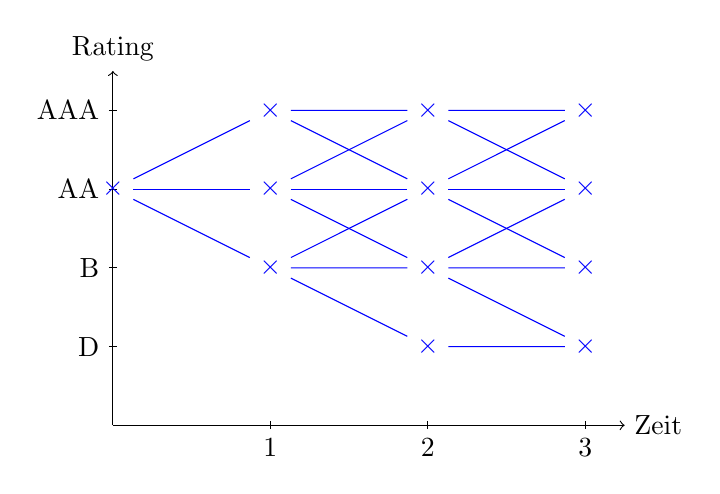
\begin{tikzpicture}
				\draw[->] (0,0) -- (6.5,0) node[right] {Zeit};
				\draw[->] (0,0) -- (0,4.5) node[above] {Rating};
				
				\draw (-0.05,1) node[left] {D} to (0.05,1);
				\draw (-0.05,2) node[left] {B} to (0.05,2);
				\draw (-0.05,3) node[left] {AA} to (0.05,3);
				\draw (-0.05,4) node[left] {AAA} to (0.05,4);
				
				\draw (2,0.05) -- (2,-0.05) node[below] {1};
				\draw (4,0.05) -- (4,-0.05) node[below] {2};
				\draw (6,0.05) -- (6,-0.05) node[below] {3};
				
				\node[blue] at (0,3) (a3) {$\times$};
				
				\node[blue] at (2,2) (b2) {$\times$};
				\node[blue] at (2,3) (b3) {$\times$};
				\node[blue] at (2,4) (b4) {$\times$};
				
				\node[blue] at (4,1) (c1) {$\times$};
				\node[blue] at (4,2) (c2) {$\times$};
				\node[blue] at (4,3) (c3) {$\times$};
				\node[blue] at (4,4) (c4) {$\times$};
				
				\node[blue] at (6,1) (d1) {$\times$};
				\node[blue] at (6,2) (d2) {$\times$};
				\node[blue] at (6,3) (d3) {$\times$};
				\node[blue] at (6,4) (d4) {$\times$};
				
				\draw[blue] (a3) -- (b4) -- (c4) -- (d4);
				\draw[blue] (a3) -- (b3) -- (c3) -- (d3);
				\draw[blue] (a3) -- (b2) -- (c2) -- (d2);
				\draw[blue] (b4) -- (c3) -- (d4);
				\draw[blue] (b3) -- (c4) -- (d3);
				\draw[blue] (b3) -- (c2) -- (d3);
				\draw[blue] (b2) -- (c3) -- (d2);
				\draw[blue] (b2) -- (c1) -- (d1);
				\draw[blue] (c2) -- (d1);
			\end{tikzpicture}
		\end{center}
		\item Die Wahrscheinlichkeit, dass die Anleihe immer bei AA bleibt, ist $0.8^3=0.512$. Sei $A$ die Übergangsmatrix, also
		\begin{align}
			A = \begin{pmatrix}
				0.8 & 0.2 & 0 & 0 \\
				0.1 & 0.8 & 0.1 & 0 \\
				0 & 0.1 & 0.5 & 0.4 \\
				0 & 0 & 0 & 1
			\end{pmatrix} \notag
		\end{align}
		Die Wahrscheinlichkeiten für ein bestimmtes Rating nach 3 Perioden, wenn die Anleihe bei AA gestartet ist, ist
		\begin{align}
			\begin{pmatrix}
				0 \\ 1 \\ 0 \\ 0
			\end{pmatrix} \cdot A^3 = \begin{pmatrix}
				0.195 \\ 0.581 \\ 0.132 \\ 0.092
			\end{pmatrix} \notag
		\end{align}
		Die Wahrscheinlichkeit für ein AAA-Rating ist also 0.195.
		\item Nach 2 Perioden ist die Wahrscheinlichkeitsverteilung
		\begin{align}
			\begin{pmatrix}
				0 \\ 1 \\ 0 \\ 0
			\end{pmatrix} \cdot A^2 = \begin{pmatrix}
				0.16 \\ 0.67 \\ 0.13 \\ 0.04
			\end{pmatrix} \notag
		\end{align}
		\item Im 1. Jahr kann die Anleihe noch kein D-Rating haben, deshalb ist hier die Auszahlung von 6 sicher. Für die anderen beiden Jahre sind die erwarteten Auszahlungen
		\begin{itemize}
			\item $(0.16 + 0.67 + 0.13)\cdot 6 + 0\cdot 0 = 5.76$
			\item $(0.195 + 0.581 + 0.132)\cdot 106 + 0.092\cdot 0 = 96.248$
		\end{itemize}
		Der Preis für die Anleihe ist dann
		\begin{align}
			P &= \frac{6}{1.05} + \frac{5.76}{1.05^2} + \frac{96.248}{1.05^3} \notag \\
			&= 94.08 \notag
		\end{align}
		\item Wenn vergleichbare Anleihen 8\% Zinsen abwerfen ist der Preis der Anleihe
		\begin{align}
			P &= \frac{6}{1.08} + \frac{5.76}{1.08^2} + \frac{96.248}{1.08^3} \notag \\
			&= 86.90 \notag
		\end{align}
		Die Anleihe in (d) ist unterbewertet: Sie kostet nur 94 \EUR, ist aber 94.08 \EUR\, wert.
	\end{enumerate}
	
\end{document}